
\section{Kuvakilpailun hedelmiä}

\textit{Koska \textit{Vene}-samoajavartio ei osallistunut, heidät nostettiin kuvakilpailun tuomaristoksi. Heidän pohdintansa jälkeen tässä ovat kilpailun tulokset.}

\vspace{0.64cm}

\begin{multicols}{2}

% \vspace*{-0.32cm}
	\subsection*{3. paikka:}
\begin{center}
	\noindent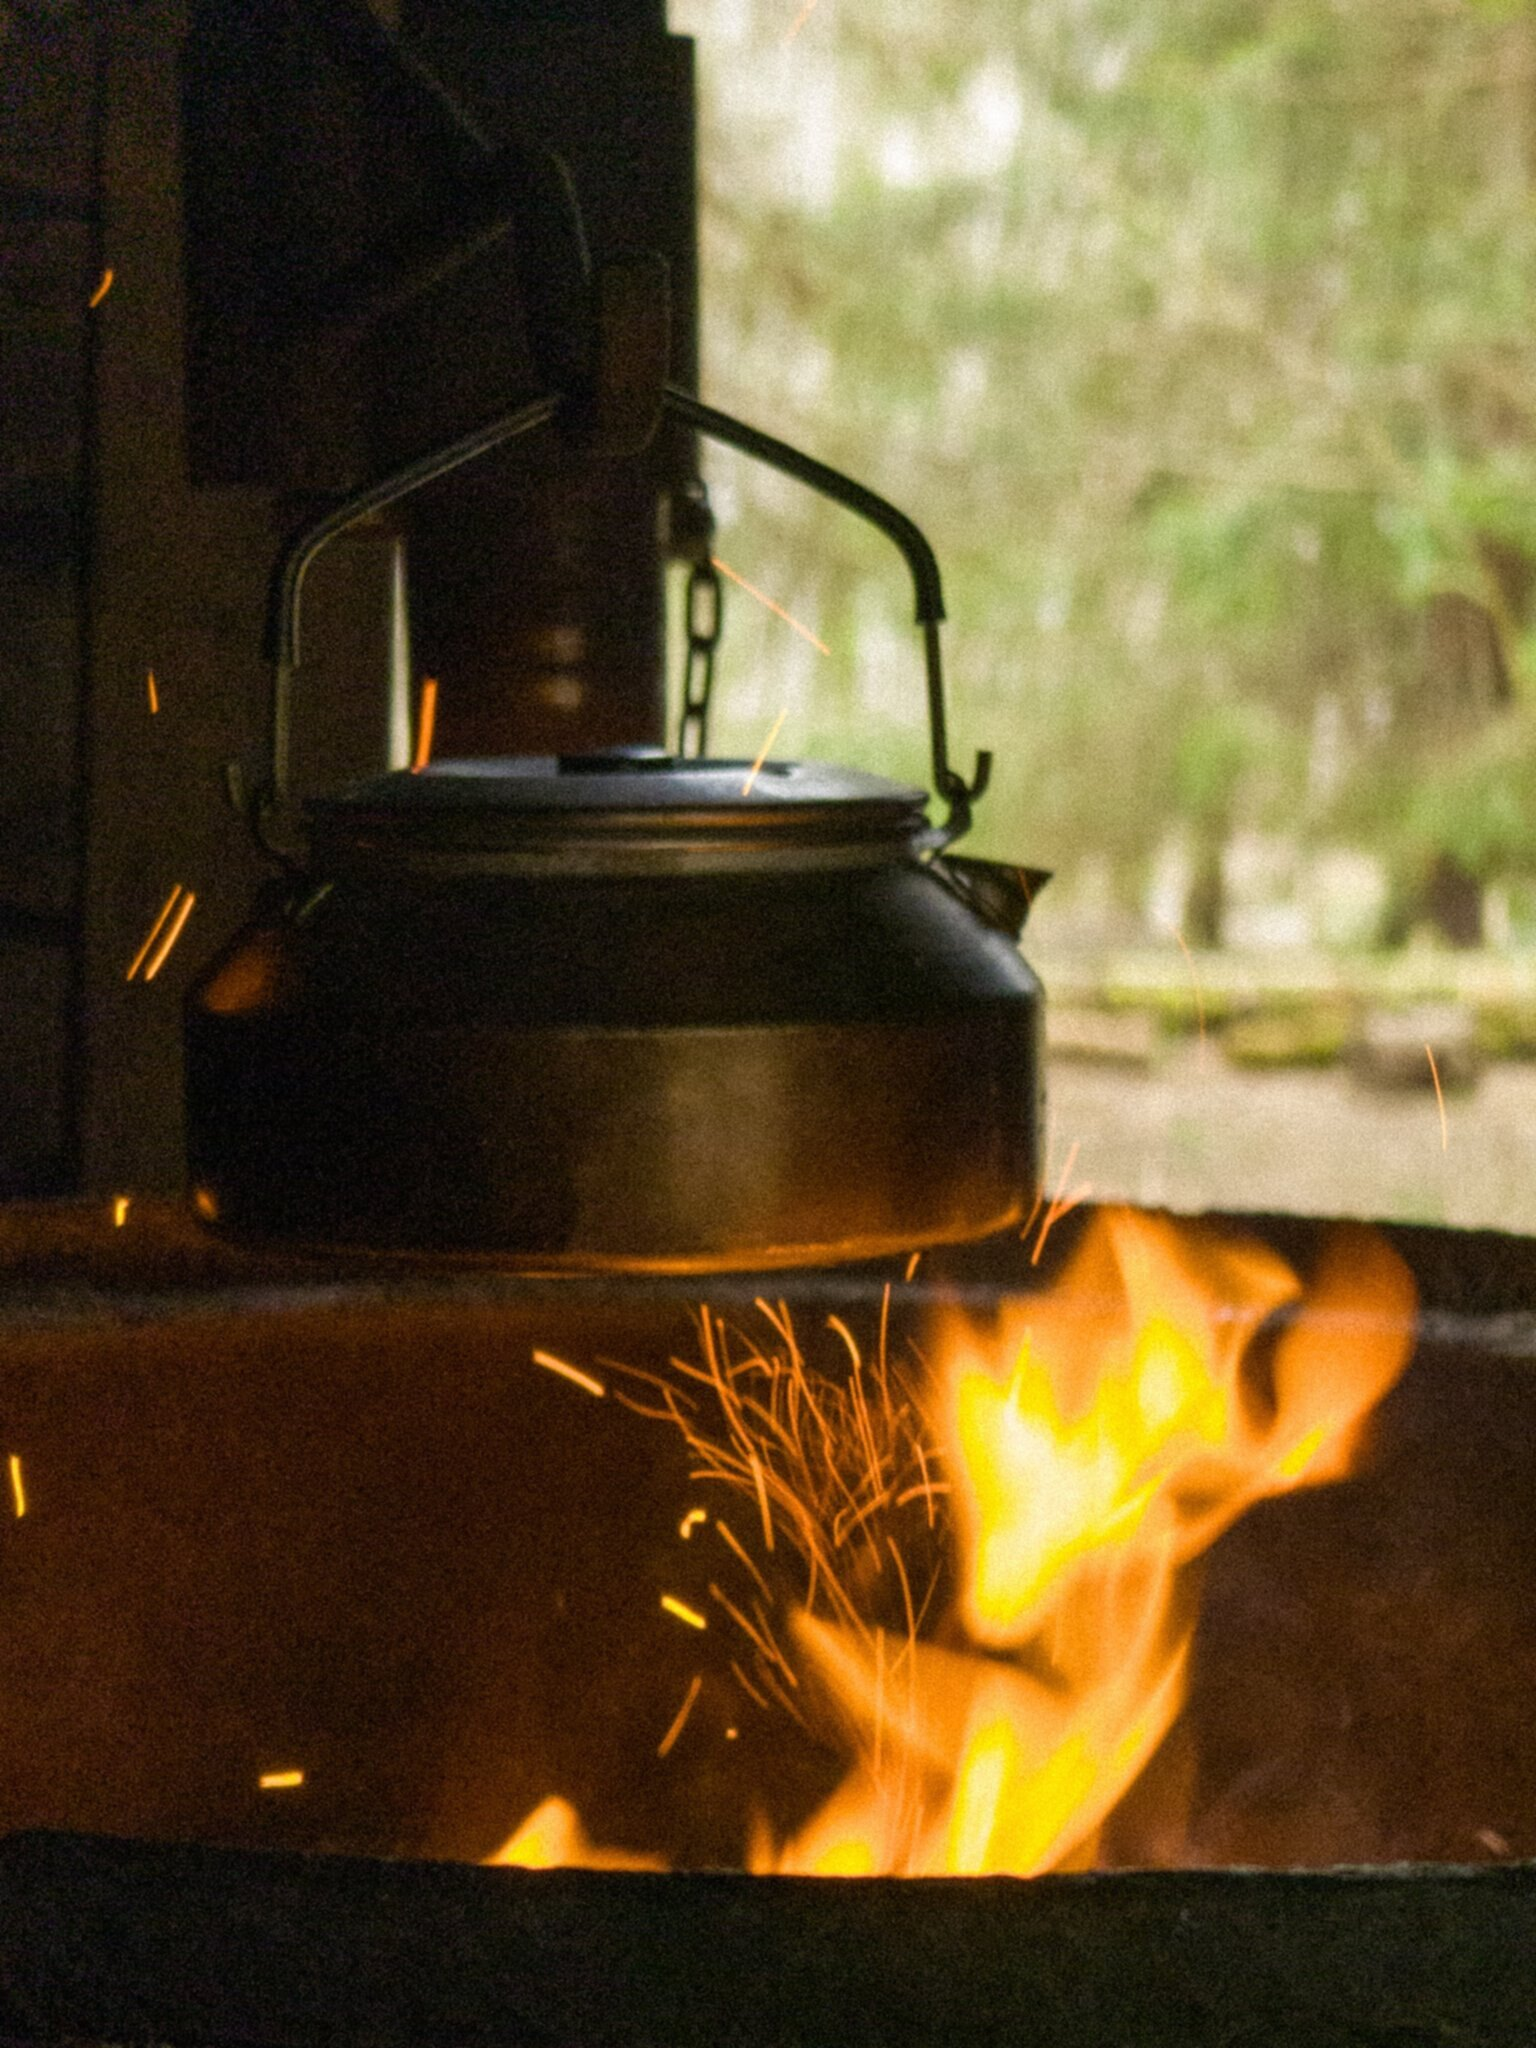
\includegraphics[height=0.9\linewidth]{assets/kuvakilpailu3}\\
	``Kahvii'' - Mikko% Niinimäki
\end{center}

\columnbreak

% \vspace*{-0.16cm}
	\subsection*{2. paikka:}
	\vspace*{0.54cm}
\begin{center}
	\noindent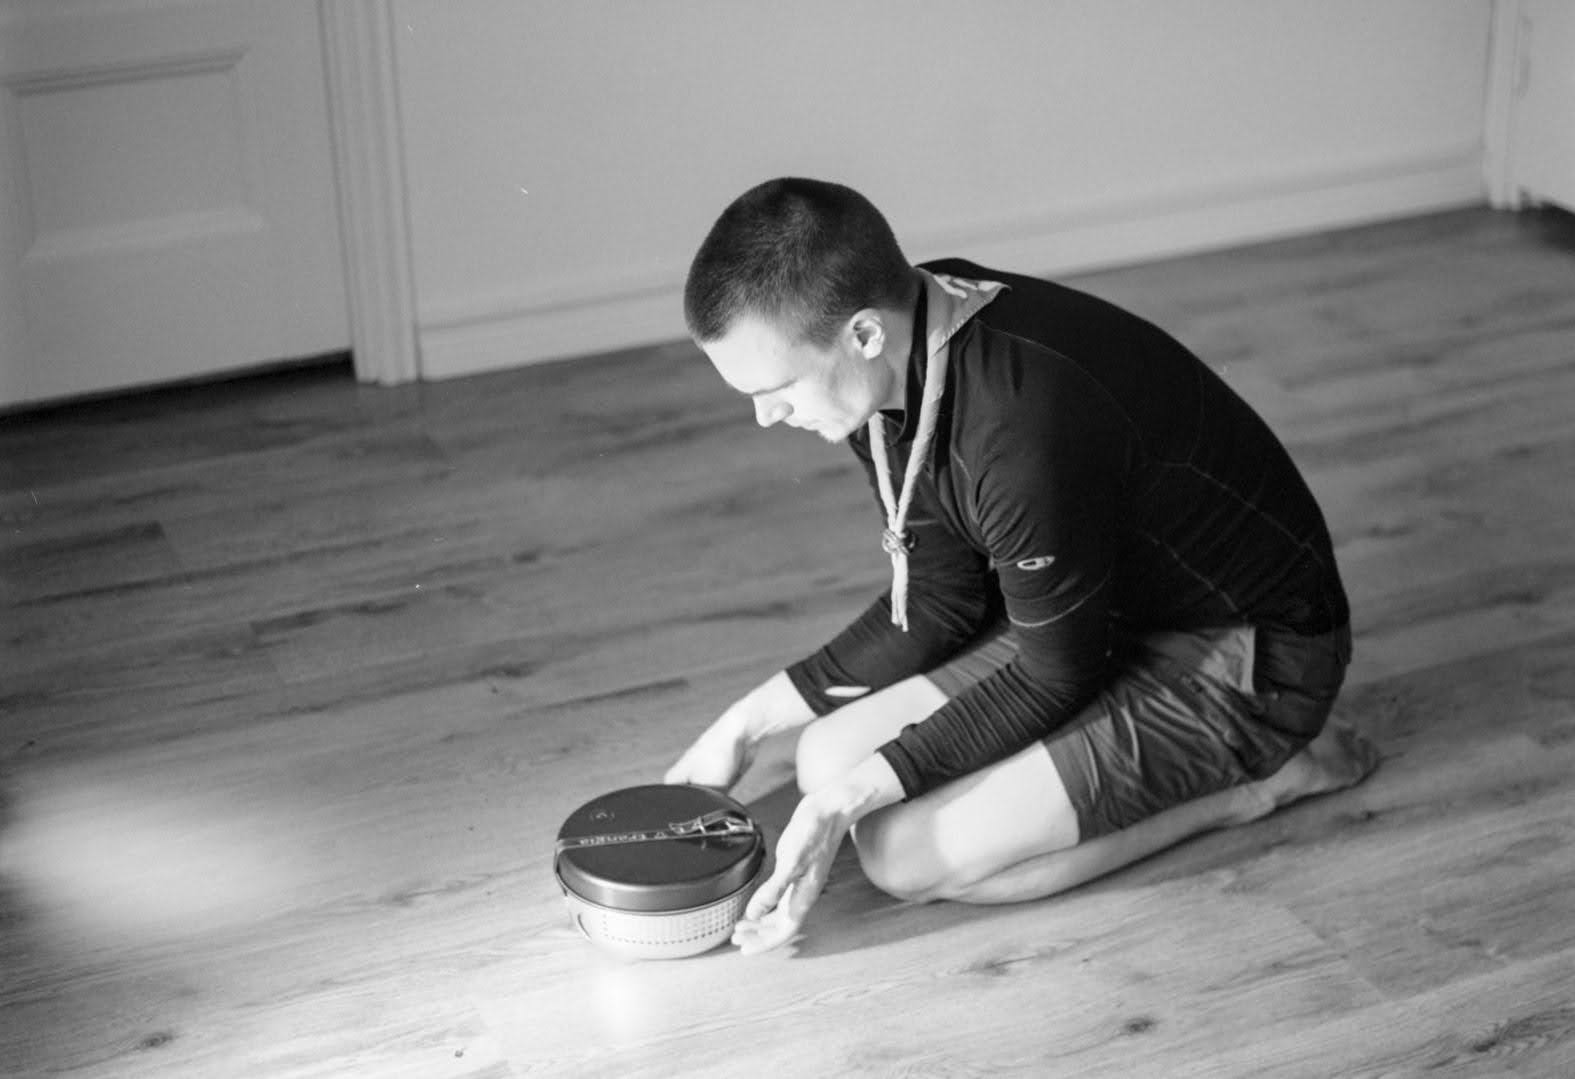
\includegraphics[width=0.99\linewidth]{assets/kuvakilpailu2}\\
	``Mies ja retkikeitin'' - Janne% Suomalainen
	\vspace*{0.54cm}
\end{center}

\end{multicols}

\begin{multicols}{2}

	\noindent Lähteet: \quad --

	\noindent Tuomariston keskiarvo: 2,5/5

	\columnbreak

	\noindent Lähteet: Poika ja pääkallo\\ \hfill - Magnus Enckell

	\noindent Tuomariston keskiarvo: 3,75/5

\end{multicols}

\begin{multicols}{2}

\noindent Kuva itsessään on oikein hieno ja se voisi sopia erinomaisesti Tassuun esim.
artikkelin kuvitukseksi. Kuva on sopivan yksinkertainen ja tunnelmallinen ja
kuvaa hyvin sitä, miltä kahvin juominen metsäretkellä tuntuu. Kuitenkin
kuvakilpailun tehtävänannon se ohittaa, sillä se ei viittaa mihinkään
taideteokseen, eikä näin ollen ole kilpailun sääntöjen mukainen.

	\columnbreak

\noindent Kuvan idea on luova ja kuvaan otettu retkikeitin myös lisää siihen
asiaankuuluvaa partiotunnelmaa. Asetelma mukailee hienosti alkuperäistä
taideteosta. Kuvan valotus on paikoittain hieman liian kirkas. Kuva on hyvin
yksinkertainen ja vaikka se ei olekaan huono asia, raati jäi kaipaamaan jotakin
elementtiä, joka olisi kiinnittänyt katsojan mielenkiinnon paremmin, minkä
vuoksi se jäi hitusen alle voittopisteiden.

\end{multicols}

\clearpage
% \vspace*{0.64cm}
\subsection*{1. paikka:}
\begin{center}
	\noindent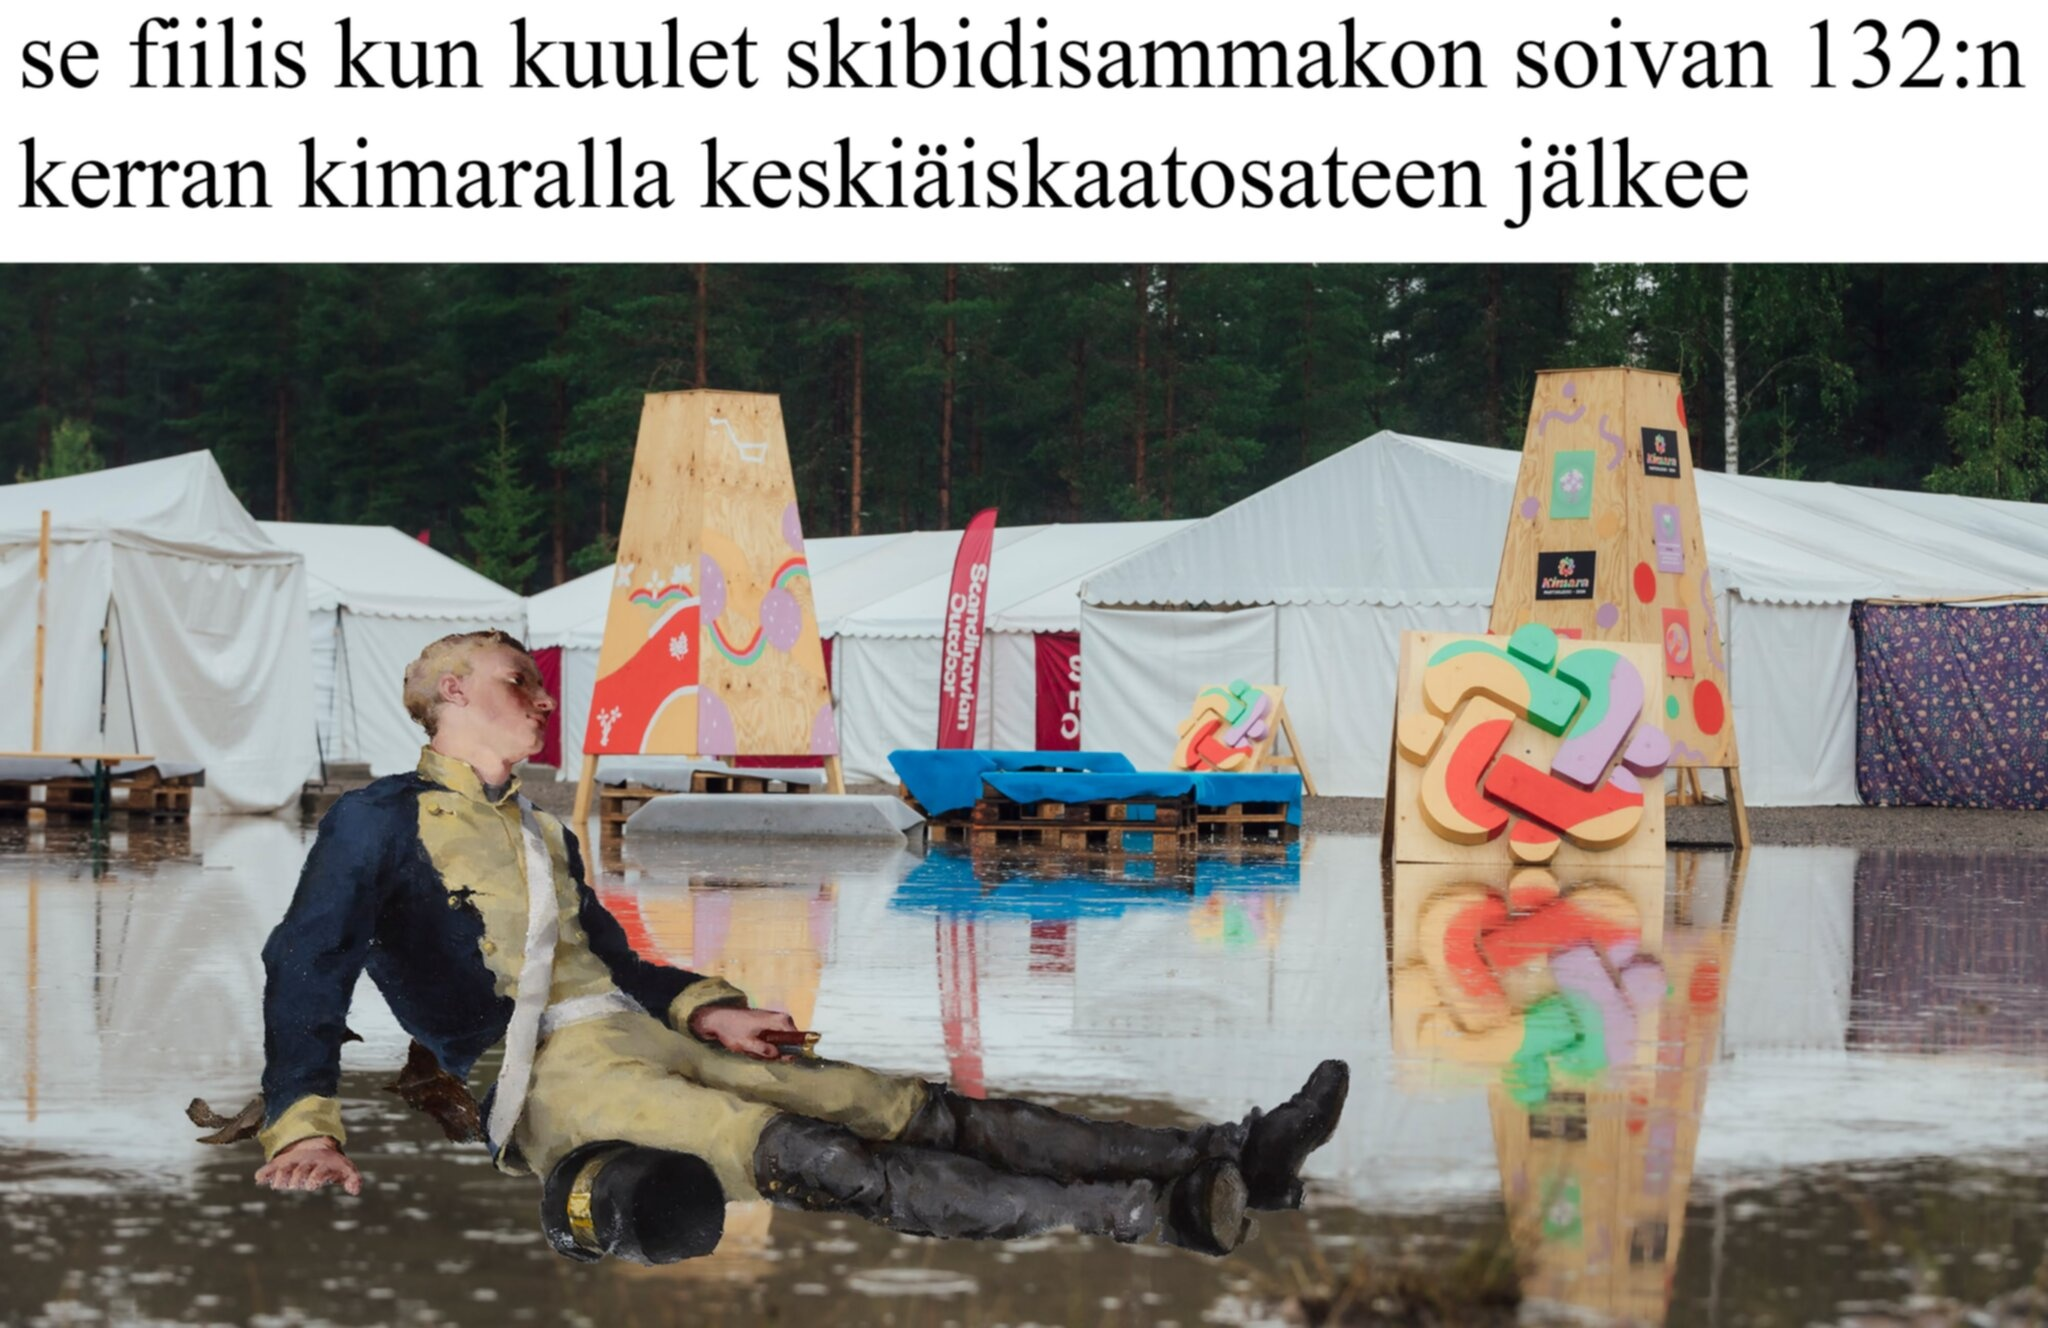
\includegraphics[width=1.0\linewidth]{assets/kuvakilpailu1}\\
	``rip bro.png'' - Alden% Forsström
\end{center}

\noindent Lähteet: \quad Haavoittunut Soturi Hangessa - Helene Schjerfbeck

\qquad\qquad Hanna Hämäläisen kuva, PäPa:n kuvapankistä

\bigskip
\noindent Tuomariston keskiarvo: 3,875/5\\
\noindent Eliaksen arvio: ``5/5 absolute cinema''

\bigskip
\noindent Kuva vetosi raatiin, sillä suurin osa pystyi samaistumaan siinä
kuvattuun tuskaan ja epätoivoon. Myös raadin iän ja kypsyyden huomioon ottaen
ei tule yllätyksenä, että meemiformaatti keräsi eniten pisteitä. Hauskuutta
kuvaan lisää se, että sen taustana on käytetty oikeaa kuvaa kuvatusta
tilanteesta. Tekijältä kuitenkin meni ohi oiva mahdollisuus käyttää numeroa
104, jolloin kuvasta olisi tullut entistä moniulotteisempi. Myös kuvatekstin
kielelliseen asuun olisi voinut panostaa enemmän. Kuva ei myöskään aukea
yleisölle, joka ei ollut Kimaralla kokemassa kuvattua tilannetta ja tästä
syystä myös tuomariston pisteiden keskiarvo laski.
